\subsection{Problema a resolver}
El siguiente problema consiste en realizar un algoritmo capaz de resolver problemas de caminos mínimos con ciertas particularidades. El mismo radica en una empresa productora de ladrillos cuyas fábricas se encuentran en distintos lugares de una provincia, al igual que sus clientes. Para transportar los ladrillos entre las fábricas y los clientes, la empresa debe encargarse de fortalecer las rutas por las que se trasladan sus camiones. Dichas rutas tienen un costo de inversión proporcional a la longitud de las mismas. Luego, la empresa desea replanificar sus recorridos a modo de minimizar los gastos que implican los fortalecimientos de las rutas a utilizar. Para ello, la empresa debe asegurarse de que exista un camino fortalecido entre cada cliente y al menos una de sus fábricas. Debe considerarse que desde todas las fábricas sale al menos una ruta, que los costos de inversión son enteros positivos, que es posible satisfacer la demanda de cada cliente y que no hay más fábricas que clientes.

Los formatos de entrada y salida del problema son los que siguen:\newline


\textbf {Formatos de entrada y salida:}\newline
\newline
La entrada contiene varias instancias del problema. La primera línea de cada instancia contiene los siguientes valores (enteros positivos, separados por un espacio):

$$F\ C\ R$$

donde \textbf{$F$} indica la cantidad de fábricas de la empresa (numeradas de 1 a \textbf{$F$}), \textbf{$C$} indica la cantidad de clientes (numerados de \textbf{$F+1$} a \textbf{$F+C$}) y \textbf{$R$} indica la cantidad de rutas de la provincia. A esta línea le siguen \textbf{$R$} líneas y cada una de ellas describe una de las rutas de la provincia. Para cada ruta, la línea correspondiente contiene los siguientes valores (enteros positivos, separados por un espacio):

$$e_{1}\ e_{2}\ l$$

donde \textbf{$e_{1}$} y \textbf{$e_{2}$} son los extremos de la ruta y \textbf{$l$} es la longitud de la misma. Los extremos de la ruta pueden ser fábricas y/o clientes y son números enteros en el rango [1,\textbf{$F+C$}]. La entrada concluye con una línea comenzada por 0.\newline

La salida debe contener una línea por cada instancia de entrada. Esta línea debe contener los siguientes valores (separados por un espacio):

$$L\ k\ e_{1}^1\ e_{2}^1\ e_{1}^2\ e_{2}^2\...\ e_{1}^k\ e_{2}^k$$

donde \textbf{$L$} es el costo total de la solución (la suma de las longitudes de las rutas utilizadas), $k$ es la cantidad de rutas utilizadas en la solución y $e_{1}^i$ y $e_{2}^i$ son los extremos de la $i$-ésima ruta utilizada, para $i\ \in$ [1,$k$].\newline

En lo que sigue, presentaremos dos ejemplos del problema a resolver:
\begin{itemize}
\item {\large{\textbf{Ejemplo 1:}}}\newline
\newline
En el ejemplo que sigue, decidimos mostrar un clásico caso del problema. En éste, se puede observar que, si bien existe más de una ruta entre cada cliente y alguna fábrica, la solución devuelve una sola ruta para cada uno de ellos.\newline
\newline
\textbf{Formato de entrada:}

$$3\ \ 5\ \ 8$$
$$1\ \ 4\ \ 40$$
$$1\ \ 5\ \ 40$$
$$4\ \ 5\ \ 100$$
$$1\ \ 6\ \ 70$$
$$6\ \ 7\ \ 100$$
$$7\ \ 2\ \ 70$$
$$2\ \ 8\ \ 40$$
$$3\ \ 8\ \ 40$$

\begin{figure}[H] %[h] Aqui [b] para button [t] para top
\begin{center}
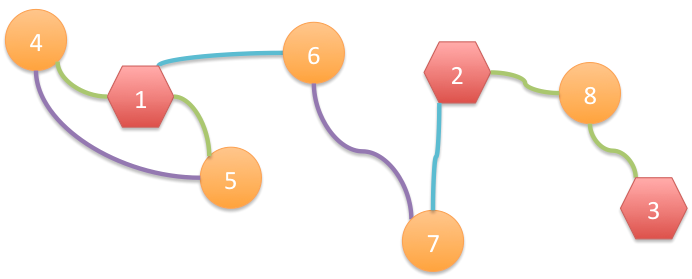
\includegraphics[width=350pt]{../imgs/ejemplo1ej3ent.jpg}
\end{center}
\fbox{\begin{minipage}[H]{90pt}
    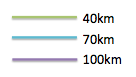
\includegraphics[width=90pt]{../imgs/leyendaej3.jpg}
  \end{minipage}}
  \hfill
  \fbox{\begin{minipage}[H]{60pt}
    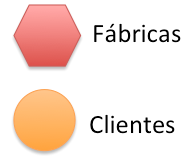
\includegraphics[width=60pt]{../imgs/leyendaformas.jpg}
  \end{minipage}}
\caption{Ejemplo 1 - entrada.}
\end{figure}

\textbf{Formato de salida:}
$$260\ \ 5\ \ 1\ \ 4\ \ 1\ \ 5\ \ 2\ \ 8\ \ 1\ \ 6\ \ 7\ \ 2$$

\begin{figure}[H] %[h] Aqui [b] para button [t] para top
\begin{center}
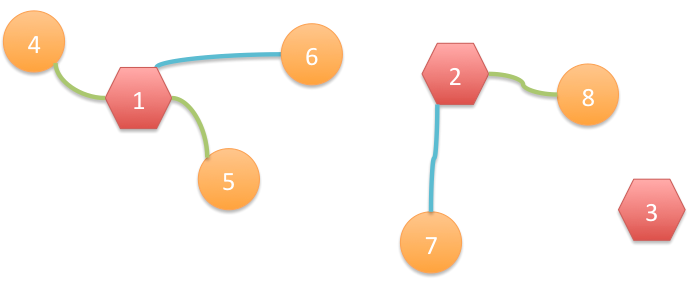
\includegraphics[width=350pt]{../imgs/ejemplo1ej3sal.jpg}
\caption{Ejemplo 1 - salida.}
\end{center}
\end{figure}
\item {\large{\textbf{Ejemplo 2:}}}\newline
\newline
En este ejemplo, puede verse que si bien todos los clientes se encuentran conectados a una fábrica de forma directa, las rutas elegidas son las indirectas dado que la suma de éstas es inferior a la otra opción. Por otra parte, puede observarse que algunas fábricas resultan inutilizables luego de la minimización de rutas, como ocurre para la fábrica nº1.\newline
\newline
\textbf{Formato de entrada:}

$$2\ \ 4\ \ 7$$
$$3\ \ 4\ \ 20$$
$$5\ \ 6\ \ 20$$
$$4\ \ 5\ \ 20$$
$$2\ \ 3\ \ 90$$
$$2\ \ 4\ \ 70$$
$$2\ \ 5\ \ 50$$
$$2\ \ 6\ \ 20$$
$$1\ \ 6\ \ 70$$

\begin{figure}[H] %[h] Aqui [b] para button [t] para top
\begin{center}
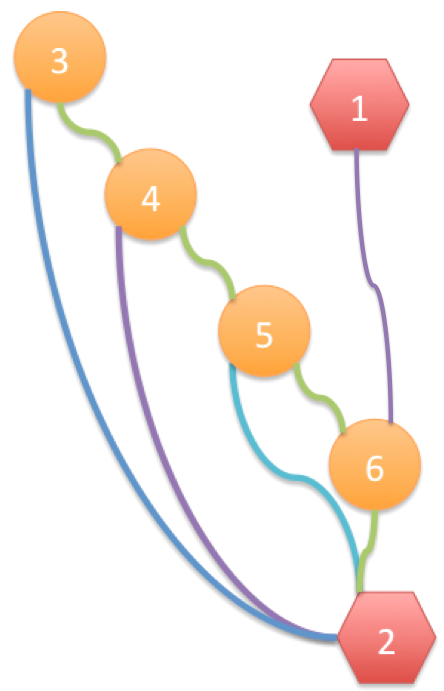
\includegraphics[width=140pt]{../imgs/ejemplo2ej3ent.jpg}
\end{center}
\fbox{\begin{minipage}[H]{70pt}
    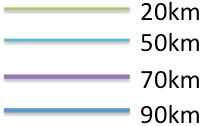
\includegraphics[width=70pt]{../imgs/leyendaej3ejmp2.jpg}
  \end{minipage}}
  \hfill
  \fbox{\begin{minipage}[H]{60pt}
    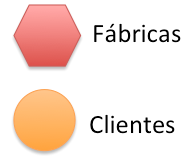
\includegraphics[width=60pt]{../imgs/leyendaformas.jpg}
  \end{minipage}}
\caption{Ejemplo 2 - entrada.}
\end{figure}

\textbf{Formato de salida:}
$$80\ \ 4\ \ 3\ \ 4\ \ 5\ \ 6\ \ 4\ \ 5\ \ 2\ \ 6$$

\begin{figure}[H] %[h] Aqui [b] para button [t] para top
\begin{center}
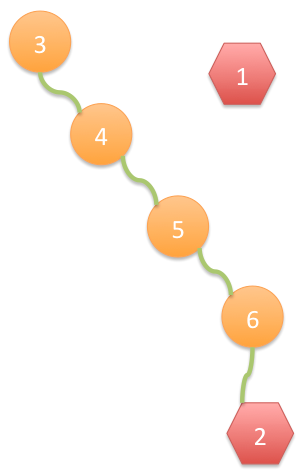
\includegraphics[width=140pt]{../imgs/ejemplo2ej3sal.jpg}
\caption{Ejemplo 2 - salida.}
\end{center}
\end{figure}
\end{itemize}


\subsection{Resolución coloquial}

Antes de explicar la resolución elegida para el problema descrito, formalicemos el modelo a utilizar:
\begin{itemize}
\item  \textbf{Nodos:} Clientes y Fábricas
\item  \textbf{Aristas:} Rutas
\item  \textbf{Pesos de las aristas:} Longitud
\end{itemize}

Luego, cuando hablemos de \textbf{Grafo}, nos vamos a estar refiriendo a una provincia que contiene clientes, fábricas y rutas.\newline

Para resolver este problema, optamos por la utilización de un algoritmo encargado de hallar un Árbol Generador Mínimo. Esto se debe a que buscamos minimizar el costo de reparación de las rutas siempre que se respete la restricción de que todos los clientes se mantengan conectados con al menos una fábrica. Luego, buscamos minimizar el peso de las aristas del grafo.\newline

Al idealizar la resolución del problema, nos encontramos con que puede no existir un camino entre todo par de vértices (un grafo no conexo). Esto nos impidió utilizar los algoritmos vistos en clase dado que aplican sobre grafos conexos. Para solucionar dicho inconveniente, optamos por crear un nodo llamado $ghost$ que se conectara con aristas de peso cero a todas las fábricas. De esta manera, nos aseguramos obtener un grafo conexo ya que todos los clientes se encuentran enlazados con al menos una fábrica y unimos todas las componentes conexas.\newline

Una vez insertado el nodo $ghost$, se ejecuta el algoritmo de $Kruskal$ a fin de hallar un árbol generador mínimo. Luego, la suma de las longitudes de todas las rutas es la menor. Posteriormente, procedemos a eliminar el nodo $ghost$, obteniendo, así, un conjunto de componentes conexas con al menos una fábrica cada una y cuyas sumas de las longitudes de rutas a reparar es la menor posible.\newline

El pseudocódigo que resuelve el problema es el siguiente:\newline

\begin{algorithm}[H]
	\SetAlgoLined
	\caption{Minimización de Caminos entre Fábricas y Clientes}
	\KwIn{Grafo $G$, Precios $ps$}
	\KwOut{Grafo}
	NodoFabrica $ghost$\\
	Agregar(Nodos($G$),$ghost$)\\
	\ForAll{$v \in$ Nodos($G$)}{
		\If{esFabrica($v$) $\land\ v\ \neq\ ghost$}{ \\
			Agregar(aristas($G$),$<v$,$ghost>$)\\
			$ps$[$v$,$ghost$] = $0$ \\
		}
	}
	Kruskal($G$,$ps$) \\
	Filtrar($G$,$ghost$) \\
	\textbf{devolver} $G$	
\end{algorithm}

\begin{algorithm}[H]
	\SetAlgoLined
	\caption{Filtrar}
	\KwIn{Grafo $G$, Nodo $ghost$}
	\ForAll{$v \in$ Nodos($G$)}{
		\If{$v$ \textbf{incide con} $ghost$}{ \\
			\textbf{Eliminar arista} $<v$,$ghost>$\\
		}
	}	
\end{algorithm}

donde $Agregar(Nodos(G),x)$ agrega el nodo $x$ a los nodos de $G$. Por otro lado, $esFabrica(v)$ es una función que devuelve $true$ si $v$ es una fábrica, caso contrario devuelve $false$.

\subsection{Demostración de correctitud}

Demostremos que el algoritmo planteado es correcto. Para ello, veamos que \textbf{se fortalecen las rutas necesarias al menor costo posible}. Donde \textbf{rutas necesarias} hace referencia a un conjunto de rutas tal que existe al menos un camino fortalecido entre un cliente y una fábrica. Por otro lado, \textbf{menor costo posible} hace alusión a que la sumatoria de todos los costos sea el menor posible.\newline

Por un lado, sabemos que \textbf{es posible satisfacer la demanda de todos los clientes} implica que para todo cliente existe un camino que lo une a una fábrica $[1]$.  \newline
\begin{figure}[H] %[h] Aqui [b] para button [t] para top
\begin{center}
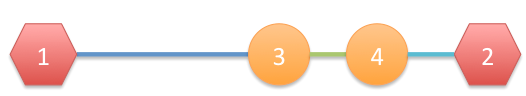
\includegraphics[width=230pt]{../imgs/demo3-1.jpg}
\end{center}
%\fbox{\begin{minipage}[H]{70pt}
%  \end{minipage}}
  \hfill
  \fbox{\begin{minipage}[H]{90pt}
    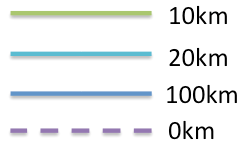
\includegraphics[width=90pt]{../imgs/leyendademo3.jpg}
  \end{minipage}}
  \caption{Ejemplo que muestra que todo cliente se une con al menos una fábrica.}
\end{figure}
\end{itemize}

Luego, queremos probar lo siguiente:
\begin{itemize}
\item Si agregamos aristas adyacentes entre cada fábrica y un nodo $ghost$ $[2]$ y aplicamos el algoritmo de $Kruskal$, el resultado cumple que todos los clientes están conectados con todas las fábricas (pues consiste en un árbol generador) $[3]$. Por otra parte, la sumatoria de todos los costos es igual a la de la solución optima (pues las aristas agregadas tenían peso cero y $Kruskal$ selecciona la sumatoria de costos mínima).

Por lo tanto, obtenemos una solución cuyo peso es mínimo, pero que mantiene las aristas de peso cero.

\begin{figure}[H] %[h] Aqui [b] para button [t] para top
\begin{center}
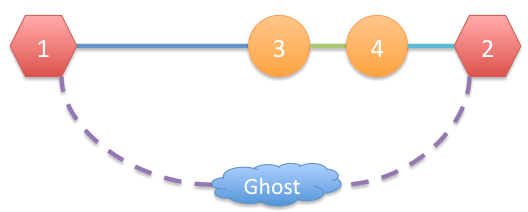
\includegraphics[width=230pt]{../imgs/demo3-2.jpg}
\caption{Ejemplo con el nodo Ghost agregado.}
\end{center}
\end{figure}
\end{itemize}


\item Luego, eliminamos las aristas que inciden en el nodo $ghost$. Dado que éstas tenían peso cero, el costo total de la solución no se ve afectado.

\begin{figure}[H] %[h] Aqui [b] para button [t] para top
\begin{center}
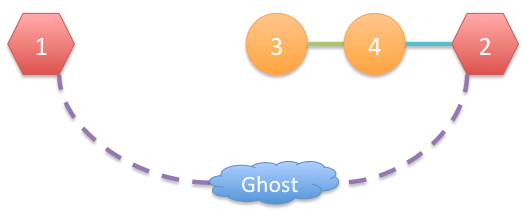
\includegraphics[width=230pt]{../imgs/demo3-3.jpg}
\caption{Ejemplo luego de aplicar el algoritmo de Kruskal.}
\end{center}
\end{figure}
\end{itemize}

\item Por último, debemos asegurarnos de que todas las componentes conexas restantes poseen al menos una fábrica. Esto se cumple ya que, por $[1]$ todas las componentes tienen al menos una fábrica, por $[3]$ todas las fábricas y clientes están conectados y, por $[2]$, las aristas eliminadas inciden sólo en fábricas, por lo que eliminarlas no descarta caminos entre clientes y éstas.

\begin{figure}[H] %[h] Aqui [b] para button [t] para top
\begin{center}

\includegraphics[width=230pt]{../imgs/demo3-4.jpg}
\caption{Ejemplo luego de eliminar las aristas de costo cero.}
\end{center}
\end{figure}
\end{itemize}

De este modo, a partir de las rutas, fábricas y clientes ingresados como parámetro de entrada, logramos obtener el conjunto de rutas cuya suma de costos es mínima logrando que cada cliente se encuentre conectado a una fábrica, siendo ésto lo que buscábamos.

\end{itemize}

\subsection{Complejidad del algoritmo}

 En esta sección, detallaremos la complejidad de nuestro algoritmo junto con la justificación de la elección de cada estructura. 

En principio, para definir el grafo ingresado por parámetro, utilizamos un $vector<Arista>$, donde $Arista$ es un struct que posee tres enteros (su peso y los nodos que conecta), y dos enteros que representan la cantidad de clientes y de fábricas. Para definir dicha estructura, reservamos ($reserve$\footnote{http://es.cppreference.com/w/cpp/container/vector/reserve}) el espacio a utilizar por el vector, siendo éste de $R + F$. Esto se debe a que, posteriormente, dicho vector almacena una suma de aristas correspondiente a la cantidad de fábricas y, de este modo, nos aseguramos de que el agregado ($push\_back$\footnote{http://es.cppreference.com/w/cpp/container/vector/push$\_$back}) de las mismas sea $\mathcal{O}(1)$. Luego, el costo de reservar dicha memoria es $\mathcal{O}(R + F)\ \leq\ \mathcal{O}(2R)$ = $\mathcal{O}(R)$, pues $F \leq R$ (por enunciado\footnote{Enunciado: "Se sabe que desde todas las fabricas sale al menos una ruta, que es posible satisfacer la demanda de cada cliente, y que no hay mas fabricas que clientes"}). De este modo, el cargado de la entrada se realiza en forma lineal respecto de la cantidad de elementos, es decir, las aristas ($R$).

 Una vez realizado esto, se comienza con la resolución del problema. Cabe aclarar que todas las funciones toman los valores por referencia, de esta manera se evitan copias innecesarias. Lo primero que realizamos es la incorporación de un nodo. Esto es constante pues consiste en sumarle uno a $cant\_nodos$ y retornar el valor obtenido. Luego, se incorporan las aristas incidentes al nodo $ghost$. Dicho proceso se realiza en tiempo lineal con respecto a la cantidad de fábricas ya que las recorre, crea una arista y la inserta en el vector (crear una arista es constante al igual que insertar el nodo pues el espacio se encontraba reservado previamente). Luego, la cantidad de rutas pasa a ser $R+F$.

 Posteriormente, se prosigue aplicando el algoritmo de $Kruskal$ cuyo costo temporal es $\mathcal{O}(m^*log(n))$\footnote{Dicha complejidad se encuentra detallada en la sección $2.1$ dado que se utilizó exactamente el mismo algoritmo.} donde $m$ = $R+F$ y $n$ = $F+C$.

 Luego del algoritmo de $Kruskal$, se realiza el llamado a la función $filtrar$. Ésta comienza con la función $reserve$ ($\mathcal{O}(n)$)\footnote{http://www.cplusplus.com/reference/vector/vector/reserve/} que reserva la cantidad de rutas menos la cantidad de fábricas, luego $R+F$-$F$ = $R$ lugares en el vector. A continuación, se recorren todas las aristas $R+F$ almacenando, en cada paso, las arista no incidentes en el nodo $ghost$ en el vector creado anteriormente. Dicha comparación es constante ya que sólo se accede a un par de aristas. Por último, se le resta uno a la cantidad de nodos ($\mathcal{O}(1)$) permitiéndonos concluir que la complejidad final de esta función resulta $\mathcal{O}(R+F)$ = $\mathcal{O}(R)$.

 Finalmente, podemos concluir que la complejidad resulta $\mathcal{O}(R)$ + $\mathcal{O}(F)$ + $\mathcal{O}((R+F)log(F+C))$ + $\mathcal{O}(R)$ + $\mathcal{O}(R)$ =  $\mathcal{O}((R+F)log(F+C))$ = $\mathcal{O}(2^*R^*log(2C))$ = $\mathcal{O}(2^*log(2)^*R^*log(C))$ = $\mathcal{O}(R^*log(C))$ dado que $F \leq C \leq R$.


\subsection{Instancias posibles}
Para verificar la correctitud de nuestro programa, dispusimos variar estratégicamente las instancias de entrada al ejecutarlo.
\begin{itemize}

\item En primer lugar, ingresamos una instancia que consideramos base. Ésta consiste en una única fábrica conectada a un cliente. Dado que no es posible ingresar el carácter 0 por ser el indicador del final del archivo, no pueden existir casos con valores menores a éste.
De este modo, logramos evaluar un tipo de caso borde.\newline
\textbf{Parámetro de entrada:} $$1\ \ 1\ \ 1$$
$$1\ \ 2\ \ 10$$
\textbf{Parámetro de salida:} $$10\ \ 1\ \ 1\ \ 2$$


\item Por otra parte, probamos ingresando dos clientes y una fábrica interconectados entre sí. El objetivo de esta instancia es ver que nuestro algoritmo elige, efectivamente, el camino más corto sin importar de qué modo une a los clientes con la fábrica ya que ésto resulta indistinto siempre que la componente conexa la contenga. \newline
\begin{figure}[H] %[h] Aqui [b] para button [t] para top
\begin{center}
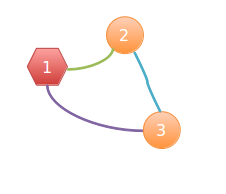
\includegraphics[width=140pt]{../imgs/caso1-ej3.png}
\end{center}
  \hfill
  \fbox{\begin{minipage}[H]{90pt}
    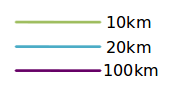
\includegraphics[width=90pt]{../imgs/leyendaformasinstancias.png}
  \end{minipage}}
\caption{Ejemplo de caso con 3 nodos}
\end{figure}
\textbf{Parámetro de entrada:} $$1\ \  2\ \  3$$
$$1\ \  2\ \  10$$
$$1\ \  3\ \  100$$
$$2\ \  3\ \  20$$																											
\textbf{Parámetro de salida:} $$30\ \ 2\ \ 1\ \ 2\ \ 2\ \ 3$$


\item También, quisimos visualizar qué ocurría cuando la entrada tenía varias soluciones posibles. De este modo, logramos ver cuál de las soluciones óptimas elegía nuestro algoritmo.\newline
\begin{figure}[H] %[h] Aqui [b] para button [t] para top
\begin{center}
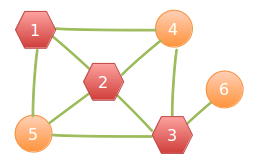
\includegraphics[width=140pt]{../imgs/caso2-ej3.png}
\end{center}
\caption{Ejemplo de varias soluciones}
\end{figure}
\textbf{Parámetro de entrada:} $$3\ \  3\ \  7$$
$$1\ \  4\ \  10$$
$$1\ \  5\ \  10$$
$$2\ \ 5\ \  10$$
$$2\ \ 4\ \  10$$
$$3\ \  5\ \  10$$
$$3\ \  4\ \  10$$
$$3\ \  6\ \  10$$
\textbf{Parámetro de salida:} $$30\ \ 3\ \ 1\ \ 4\ \ 1\ \ 5\ \ 3\ \ 6$$

\item Para finalizar, probamos un caso compuesto por varias componentes no conexas. Para ello, creamos una instancia que posee tres pares de (clientes, fábricas) no conectadas entre ellos. \newline
\begin{figure}[H] %[h] Aqui [b] para button [t] para top
\begin{center}
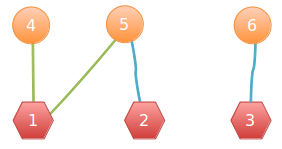
\includegraphics[width=140pt]{../imgs/caso4-ej3.png}
\end{center}
\caption{Ejemplo varias componentes conexas.}
\end{figure}
\textbf{Parámetro de entrada:} $$3\ \  3\ \  4$$
$$1\ \  4\ \  10$$
$$1\ \  6\ \  10$$
$$5\ \  2\ \  20$$
$$3\ \  6\ \  100$$																									
\textbf{Parámetro de salida:} $$40\ \ 3\ \ 1\ \ 4\ \ 1\ \ 6\ \ 5\ \ 2$$

\end{itemize}


De este modo, logramos abarcar los casos límite en los que la implementación pudiera haber encontrado algún problema. Dado que los resultados obtenidos fueron los esperados, determinamos que para todas las instancias válidas posibles de entrada nuestra implementación resulta correcta.


\subsection{Experimentación}
Para las pruebas de complejidad empírica, generamos instancias aleatorias de grafos alterando la cantidad de nodos y aristas. Estas instancias fueron generadas en $C++$ con la función $rand()$. La cantidad de grafos generados se comprendió entre 200 y 100000, agregando de a 200 en cada iteración. Las mediciones de tiempo en nanosegundos se realizaron con la función $high\ resolution\ clock$\footnote{http://en.cppreference.com/w/cpp/chrono/high\_resolution\_clock} de la librería $Chrono$ de $C++$. Debido a que éstas fueron realizadas en nanosegundos, las pruebas cuyo tamaño de la entrada era menor a 200 se realizaba en mayor tiempo que las instancias más grandes pues el procesador le otorga más atención al no realizar cambio de contexto. De este modo, logramos medir las pruebas de nuestro algoritmo para comprobar que la complejidad correspondiera con la mencionada anteriormente.

Las funciones de complejidad con las que se compararon nuestros gráficos de tiempo fueron ajustadas por algoritmos matemáticos (proporcionados por \textbf{sci davis}). Dichos algoritmos se encargaron de multiplicarle y sumarle constantes a las funciones con el fin de que éstas se ajustaran a nuestros resultados sin modificar el comportamiento de las funciones utilizadas para comparar.

El algoritmo generador de instancias utilizado garantiza que siempre existe al menos una fábrica conectada directa o indirectamente a un cliente, de forma tal que la instancia no se vuelva inválida.
\newpage
En primer lugar, generamos grafos aleatorios variando la cantidad de nodos y dejando la cantidad de aristas en un valor fijo. Este valor es un porcentaje de la cantidad máxima de aristas que puede tener el grafo. El elegido para determinar un grafo denso fue el $50\%$ de la cantidad máxima de aristas que puede tener el grafo. La cantidad de nodos que representan fábricas es el $50\%$.

\begin{figure}[H]
\begin{center}
	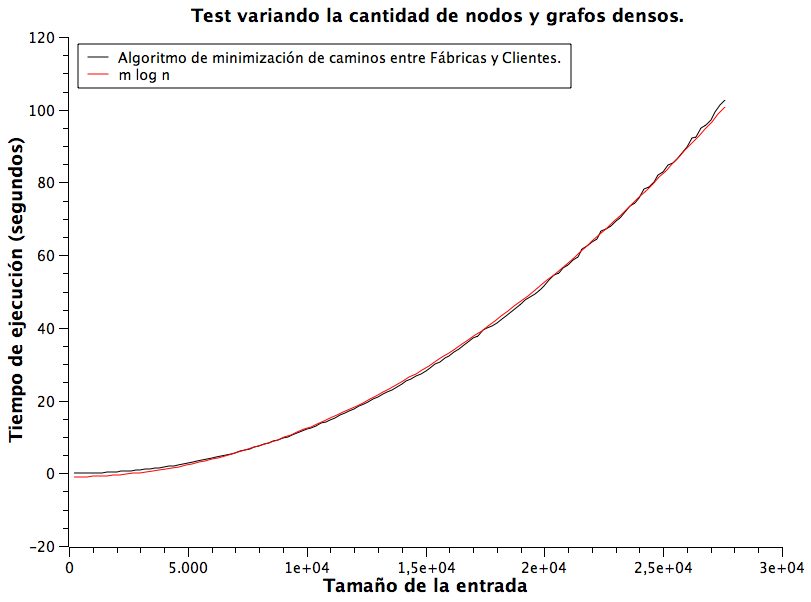
\includegraphics[width=350pt]{../tests/ej3/EJ3-nodo-var-denso.png}
\end{center}
\end{figure}

En este caso, se puede apreciar cómo la complejidad se adapta perfectamente a los valores de entrada.\\
La función utilizada para aproximar nuestros valores resultantes luego de las distintas ejecuciones fue $$a*(((20*(x*(x-1)/2)) / 100) + log(x)) + b$$.
En este caso, los valores que aproximan la función a nuestros datos son:

$$desde\ x = 200\ a\ x = 27.600 $$
$$a  = 1,33661247156849e-06$$
$$b  = -1,01492247788281 $$

Luego, generamos un lote de pruebas para grafos livianos, a diferencia de los anteriores, éstos se conforman por un $5\%$ de aristas y $5\%$ de nodos que representan fábricas.

\begin{figure}[H]
	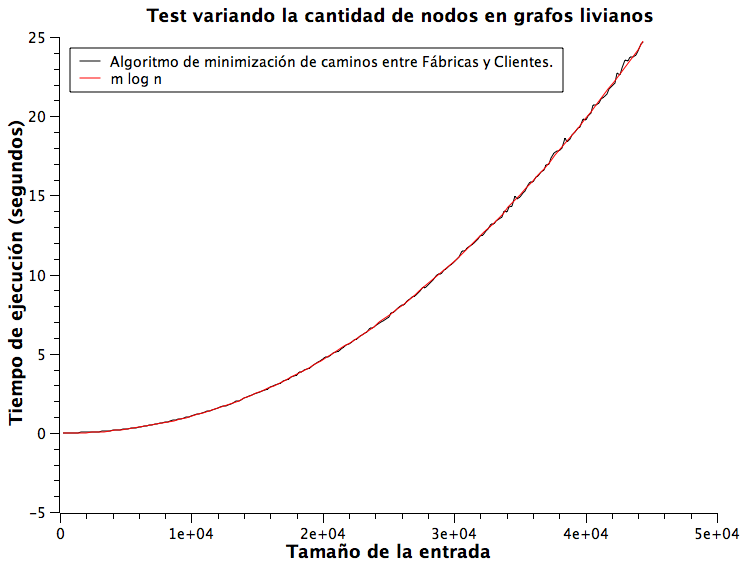
\includegraphics[width=350pt]{../tests/ej3/EJ3-nodo-var-liviano.png}
%\end{center}
\end{figure}

Al igual que en el caso anterior, se puede apreciar cómo la complejidad se adapta perfectamente a los valores de entrada. Con respecto al caso anterior, los tiempos de ejecución son más rápidos con lo cual se pudo realizar una mayor cantidad de pruebas. Esto deja en evidencia que la cantidad de aristas impacta directamente en la complejidad, tal como mostramos en el análisis del mismo.\\
La función utilizada para aproximar nuestros valores resultantes luego de las distintas ejecuciones fue $$ a*(((20*(x*(x-1)/2)) / 100) + log(x)) + b $$.
En este caso, los valores que aproximan la función a nuestros datos son:

$$desde\ x = 200\ a\ x = 44.400 $$
$$a  = 2,70030174291421e-08$$
$$b  = -0,0228951001523759 $$


\newpage
Luego, generamos un lote de grafos cuya cantidad de nodos está fija, variando la cantidad de aristas entre 1 y 100$\%$ sobre la capacidad máxima de aristas que puede soportar el grafo. La cantidad de nodos que elegimos para este grafo es de $3000$. La cantidad de fábricas en este caso es del $20\%$.

\begin{figure}[H]
\begin{center}
	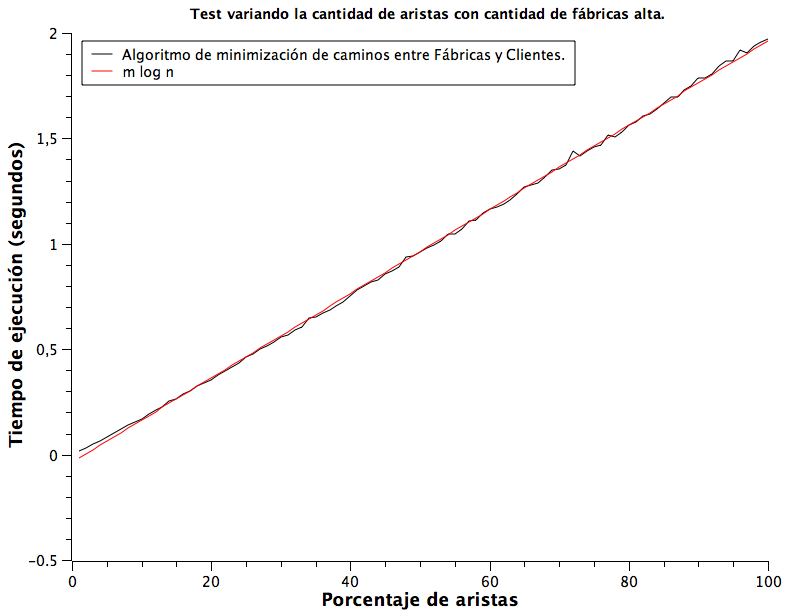
\includegraphics[width=350pt]{../tests/ej3/EJ3-r-var-denso.png}
\end{center}
\end{figure}

Nuevamente, podemos ver que la complejidad se adapta a los valores de entrada. Debido a que la función de complejidad fija la parte logarítmica, los valores resultantes se parecen a una función lineal, lo cual tiene sentido ya que la única variable que se modifica a lo largo de las pruebas es lineal.\\
La función utilizada para aproximar nuestros valores resultantes luego de las distintas ejecuciones fue $$a*((x*(3000*(3000-1)/2))/100)*log(3000)+b $$.
En este caso, los valores que aproximan la función a nuestros datos son:

$$desde\ x = 1\ a\ x = 100 $$
$$a  = 1,27748699850107e-07$$
$$b  = -0,0359196477978645 $$

\newpage
Luego, generamos un lote igual al anterior excepto por el porcentaje de fábricas, esto lo hicimos para ver si la complejidad se veía afectada por la cantidad de conexiones de nodos fantasmas que el programa hace. El porcentaje de fábricas para este caso es del $1\%$.

\begin{figure}[H]
\begin{center}
	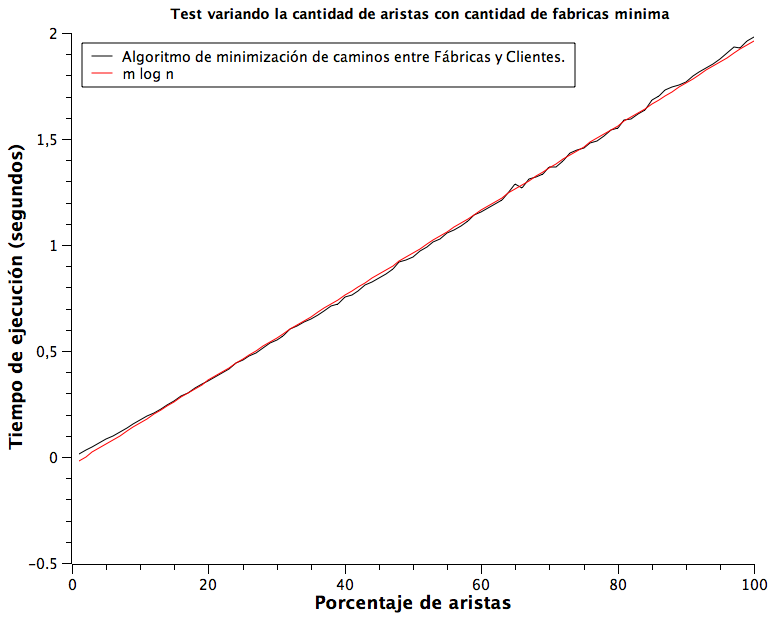
\includegraphics[width=350pt]{../tests/ej3/EJ3-r-var-liviano.png}
\end{center}
\end{figure}

Podemos ver que la función de complejidad se adapta a los valores medidos y podemos concluir que la cantidad de fábricas no modifica la complejidad del algoritmo, siendo los tiempos del gráfico iguales al anterior.\\
La función utilizada para aproximar nuestros valores resultantes luego de las distintas ejecuciones fue $$ a*((x*(3000*(3000-1)/2))/100)*log(3000)+b$$.
En este caso, los valores que aproximan la función a nuestros datos son:

$$desde\ x = 1\ a\ x = 100$$
$$a  = 1,28059038055647e-07$$
$$b  = -0,038836147808835$$

\newpage 
Finalmente, veamos un caso en el que varía la cantidad de nodos que representan fábricas para ver si influye en los tiempos de ejecución del algoritmo. Para ello, creamos dos lotes. En el primero, que definimos como denso, la cantidad de aristas está en función de la cantidad de nodos, siendo ésta del $20\%$. En el segundo lote, que definimos como liviano, pusimos la mínima cantidad de aristas, siendo ésta la mínimo para garantizar que las instancias de los problemas fueran válidas. La cantidad de nodos de este grafo es de $3000$.

\begin{figure}[H]
\begin{center}
	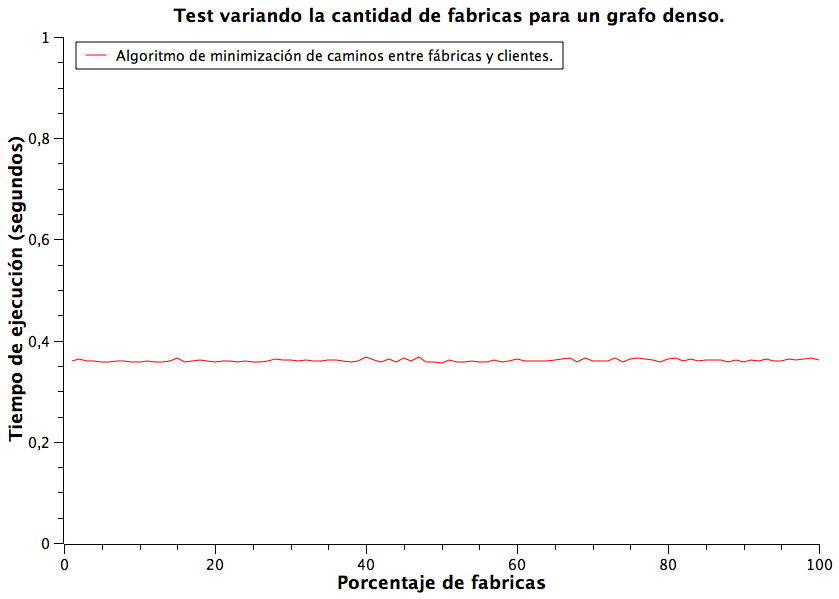
\includegraphics[width=370pt]{../tests/ej3/EJ3-f-var-denso.png}
\end{center}
\end{figure}

\begin{figure}[H]
\begin{center}
	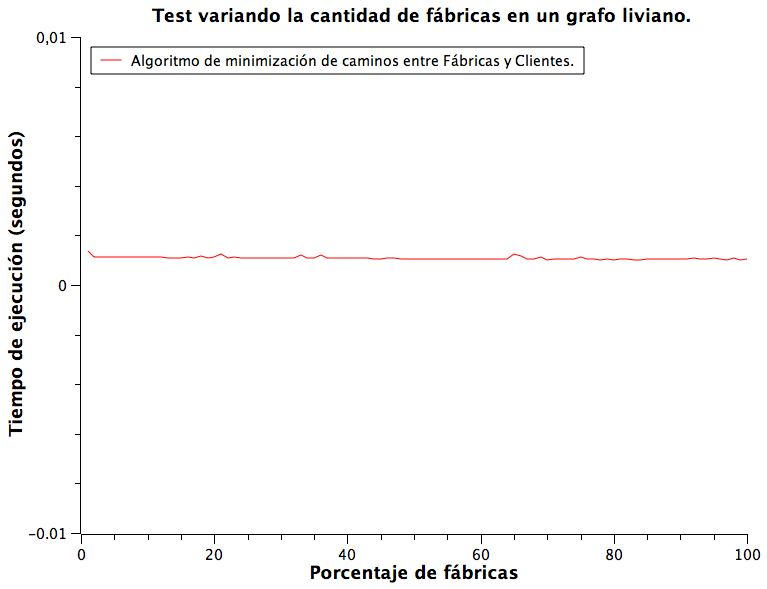
\includegraphics[width=370pt]{../tests/ej3/EJ3-f-var-liviano.png}
\end{center}
\end{figure}
